\section {Preliminary Tests with Cosmic Rays and Results} 

The Hamamatsu R7899 photomultiplier tubes have been chosen to provide highest possible gain. They been tested using a stable, fast LED source that is capable of generating light in a wide range of intensity proportional to the voltage applied to the LED. Gain equalization of phototubes establishing values for High Voltages was done based on LED calibration for sides A and B. The high voltages have been chosen such that on average $\bar{N}_{pe} \approx 106$ p.e. signal correspond to the same channel 106.5 in ADC (pedestals subtracted). The prototype was tested on cosmic rays. The test setup (still available) is comprised of two scintillating counters to generate a trigger signal and a 2" thick Tungsten plate that serves as an absorber to reduce low energy background. Preliminary cosmic ray tests results are shown on Figures \ref{fig:CosmicsA} for side A (direct coupling) and \ref{fig:CosmicsB} for side B (light guide coupling). The obtained MIP signals were fitted by Vavilov’s distribution function. In Figure \ref{fig:CosmicsA11} fit results are shown for channel A11. On ADC spectra (pedestals subtracted) the peak position in average is (70 $\pm$ 4.5) channel which brings to $\bar{N}_{pe} \approx 106$ p.e. as of calibration data. The average energy deposition by MIP in a single channel is $\bar{\Delta E}_{MIP} \sim $ 1.5 MeV. Preliminary analysis of ADC spectra using calibration results have shown that the expected (GEANT 4 simulations) and measured numbers of photoelectrons per energy deposited by MIP in the scintillating fibers agree with each other: $\bar{n}_{p.e.} = (71 \pm 4.5)$ p.e./MeV.\\
This validated our construction technique of the prototype with direct coupling between fibers and photomultipliers since this readout scheme provided better results and is more cost effective (less surface polishing is required).

\begin{figure}[h]
\centering
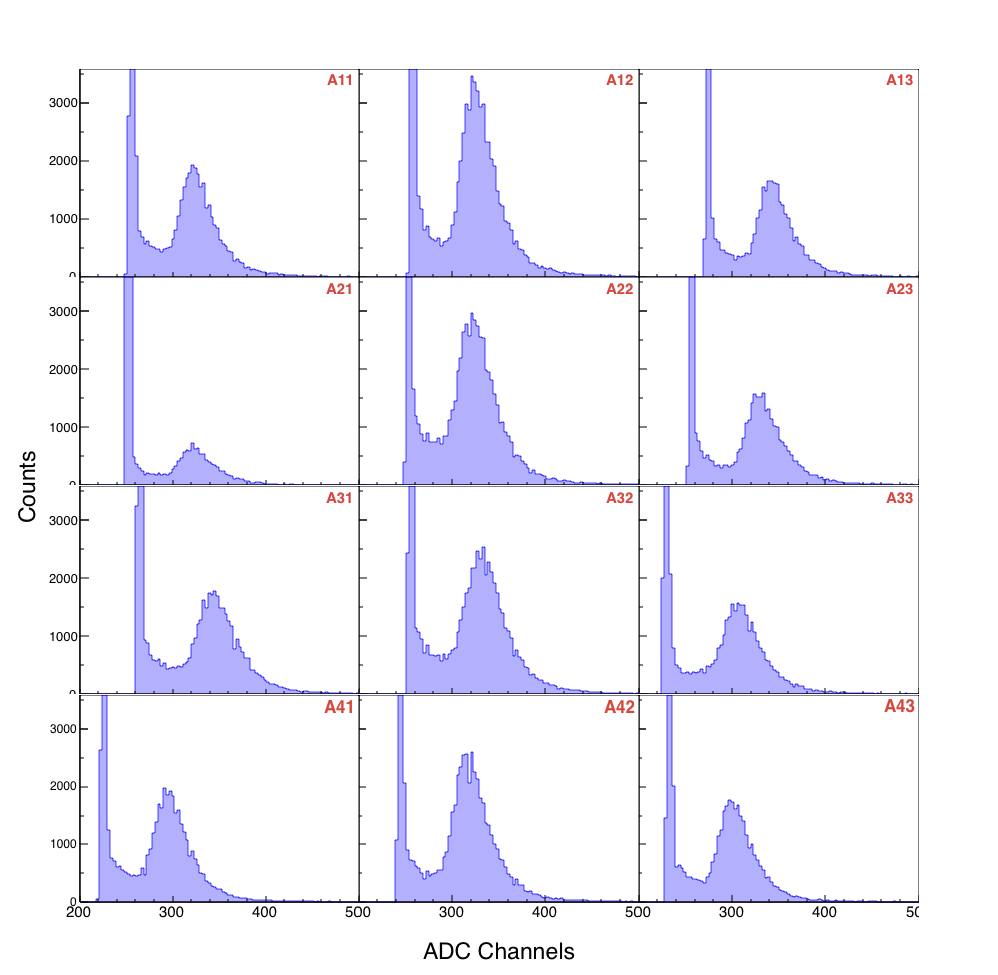
\includegraphics[width=0.95\linewidth]{images/Fig12a_CosmicsA.png}
\caption{Cosmic ray tests. Raw ADC spectra for each of 12 channels for side A (Direct coupling)}
\label{fig:CosmicsA}
\end{figure}

\begin{figure}[h]
\centering
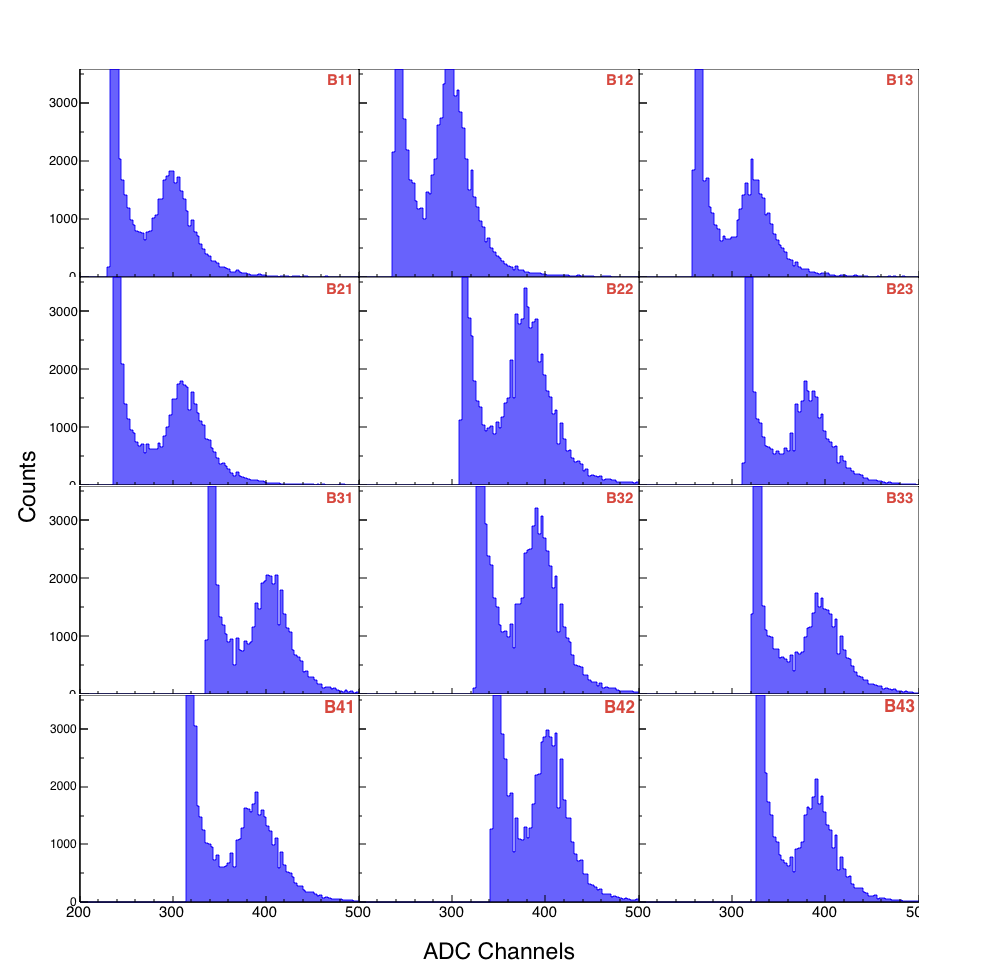
\includegraphics[width=0.95\linewidth]{images/Fig12b_CosmicsB.png}
\caption{Cosmic ray tests. Raw ADC spectra for each of 12 channels for side B (Light guide coupling)}
\label{fig:CosmicsB}
\end{figure}

\begin{figure}[h]
\centering
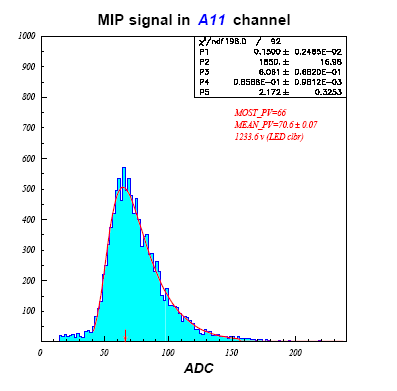
\includegraphics[width=0.9\linewidth]{images/Fig13_CosmicsA11.png}
\caption{Cosmic ray test results for channel A11 (pedestal subtracted/LED calibrated)}
\label{fig:CosmicsA11}
\end{figure}
